\section{1174006 - Kadek Diva Krishna Murti}
\subsection{Soal Teori}
\begin{enumerate}

	\item Jelaskan apa itu random forest, sertakan gambar ilustrasi buatan sendiri.
	\hfill\break
	Random forest (RF) adalah suatu algoritma yang digunakan pada klasifikasi data dalam jumlah yang besar. Klasifikasi random forest dilakukan melalui penggabungan pohon (tree) dengan melakukan training pada sampel data yang dimiliki. Penggunaan pohon (tree) yang semakin banyak akan mempengaruhi akurasi yang akan didapatkan menjadi lebih baik. Penentuan klasifikasi dengan random forest diambil berdasarkan hasil voting dari tree yang terbentuk. Pemenang dari tree yang terbentuk ditentukan dengan vote terbanyak.

	\begin{figure}[H]
	\centering
		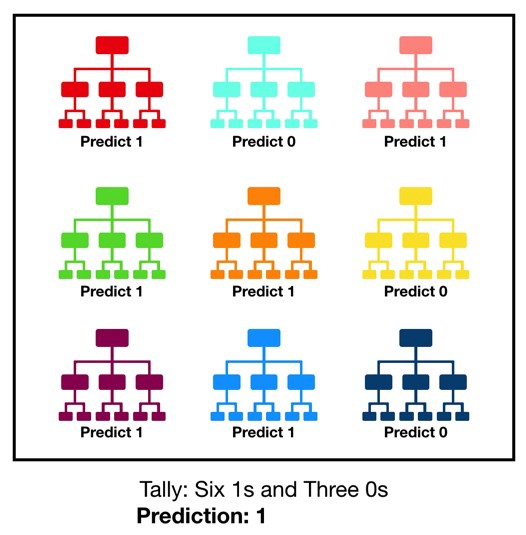
\includegraphics[width=8 cm]{figures/1174006/chapter3/soalteori/1.jpeg}
		\caption{Random Forest.}
	\end{figure}

	\item Jelaskan cara membaca dataset kasus dan artikan makna setiap file dan isi field masing-masing file.
	\hfill\break

	\begin{figure}[H]
		\centering
		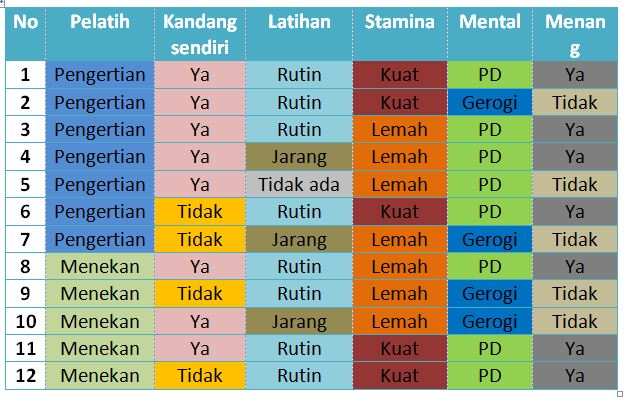
\includegraphics[width=8 cm]{figures/1174006/chapter3/soalteori/2.jpg}
		\caption{Dataset.}
	\end{figure}

	Atributte : Pelatih, kandang sendiri, latihan, stamina, mental\\
	Class     : Menang = ya atau tidak\\
	Jumlah data ada 12, terdiri dari :\\
	Ya       = 7\\
	Tidak    = 5\\
	
	\item Jelaskan apa itu cross validation.
	\hfill\break
	Cross-validation (CV) adalah metode statistik yang dapat digunakan untuk mengevaluasi kinerja model atau algoritma dimana data dipisahkan menjadi dua subset yaitu data proses pembelajaran dan data validasi / evaluasi. Model atau algoritma dilatih oleh subset pembelajaran dan divalidasi oleh subset validasi. Selanjutnya pemilihan jenis CV dapat didasarkan pada ukuran dataset. Biasanya CV K-fold digunakan karena dapat mengurangi waktu komputasi dengan tetap menjaga keakuratan estimasi.

	\begin{figure}[H]
		\centering
		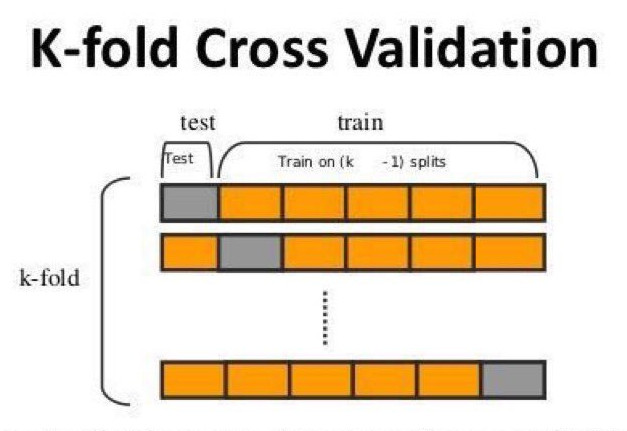
\includegraphics[width=8 cm]{figures/1174006/chapter3/soalteori/3.jpg}
		\caption{Cross Validation.}
	\end{figure}

	\item Jelaskan apa arti score 44 \% pada random forest, 27\% pada decission tree dan 29 \% dari SVM.
	\hfill\break

	44\% merupakan hasil akurasi pembelajaran mesin dengan algoritma random forest. 27\% merupakan hasil akurasi pembelajaran mesin dengan algoritma decission tree. 29\% merupakan hasil akurasi pembelajaran mesin dengan algoritma SVM.

	\item Jelaskan bagaimana cara membaca confusion matriks dan contohnya memakai gambar atau ilustrasi sendiri.
	\hfill\break
	Confusion Matrix merupakan metode untuk menghitung akurasi pada model. Confusion Matrix merepresentasikan prediksi dan kondisi sebenarnya(aktual) dari data yang dihasilkan oleh algoritma ML. Berdasarkan Confusion Matrix, kita bisa menentukan Accuracy, Precission, Recall dan Specificity. Pada pengukuran kinerja menggunakan confusion matrix, terdapat 4 (empat) istilah sebagai representasi hasil proses klasifikasi, diantaranya adalah :
	\begin{itemize}
		\item True Positive : Data positif yang terdeteksi memiliki hasil benar
		\item False Positive : Data Positif yang terdeteksi memiliki hasil salah
		\item True Negative : Data negatif yang terdeteksi memiliki hasil benar
		\item False Negative : Data negatif yang terdeteksi memiliki hasil salah
	\end{itemize}

	\hfill\break
	\begin{figure}[H]
		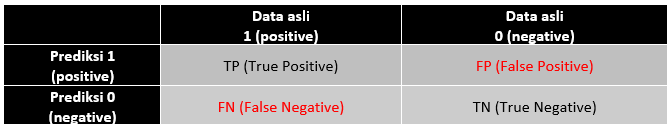
\includegraphics[width=8 cm]{figures/1174006/chapter2/teori/6.png}
		\centering
		\caption{Confusion Matrix.}
	\end{figure}

	\item Jelaskan apa itu voting pada random forest disertai dengan ilustrasi gambar sendiri
	\hfill\break
	Voting pada random forest adalah hasil penentuan klasifikasi dengan algoritma random forest berdasarkan vote paling banyak dari setiap tree yang terbentuk. Misalnya kita bingung apakah coklat X ini enak atau tidak. Maka kita bertanda ke 9 orang, pendapat mereka tentang coklat X. Jika lebih dari setengahnya (lebih dari 50\%) mengatakan bahwa coklat X rasanya enak, maka kita bisa mengatakan dia masuk ke kategori enak.
	Keputusan enak atau tidak adalah 2 kelompok yang berbeda. Sementara jumlah orang sebanyak 9 orang adalah analogi untuk decision tree yang kita kembangkan sebanyak 300 orang. Dan 50\% adalah batas (threshold) apakah ia masuk ke kategori A (enak) atau kategori B (tidak enak).

	\begin{figure}[H]
		\centering
		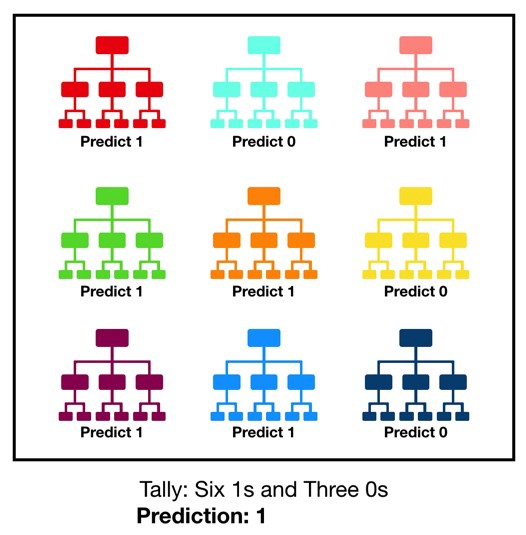
\includegraphics[width=8 cm]{figures/1174006/chapter3/soalteori/1.jpeg}
		\caption{Voting pada Random Forest.}
	\end{figure}

\end{enumerate}


\subsection{Praktek Program}
\begin{enumerate}
	\item Buat aplikasi sederhana menggunakan pandas dan jelaskan arti setiap baris kode yang dibuat (harus beda dengan teman sekelas).
	\hfill\break
	\lstinputlisting[firstline=3, lastline=8]{src/1174006/chapter3/praktek.py}
	\begin{figure}[H]
	\centering
		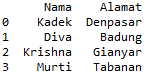
\includegraphics[width=8 cm]{figures/1174006/chapter3/soalpraktek/1.PNG}
	\end{figure}

	\item Buat aplikasi sederhana menggunakan numpy dan jelaskan arti dari setiap baris kode yang dibuat (harus beda dengan teman sekelas).
	\hfill\break
	\lstinputlisting[firstline=12, lastline=19]{src/1174006/chapter3/praktek.py}
	\begin{figure}[H]
	\centering
		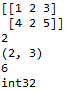
\includegraphics[width=8 cm]{figures/1174006/chapter3/soalpraktek/2.PNG}
	\end{figure}

	\item Buat aplikasi sederhana menggunakan matplotlib dan jelaskan arti dari setiap baris kode (harus beda dengan teman sekelas)
	\hfill\break
	\lstinputlisting[firstline=23, lastline=27]{src/1174006/chapter3/praktek.py}
	\begin{figure}[H]
	\centering
		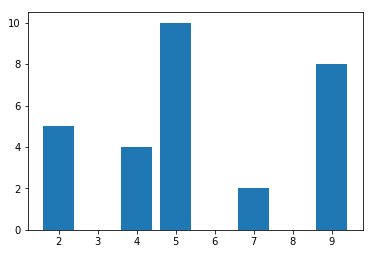
\includegraphics[width=8 cm]{figures/1174006/chapter3/soalpraktek/3.PNG}
	\end{figure}

	\item Jalankan  program  klasifikasi  Random  Fores  pada  bagian  teori  bab  ini.   Tunjukkan  keluarannya  dari  komputer  sendiri  dan  artikan  maksud  setiap  luaran yang didapatkan.
	\hfill\break
	\begin{figure}[H]
	\centering
		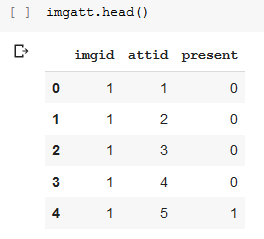
\includegraphics[width=8 cm]{figures/1174006/chapter3/soalpraktek/4-1.PNG}
	\end{figure}

	Pada id gambar 1 tidak memiliki atribut 1, 2, 3, 4, tetapi memiliki atribut 5.

	\hfill\break
	\begin{figure}[H]
	\centering
		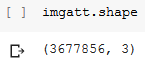
\includegraphics[width=8 cm]{figures/1174006/chapter3/soalpraktek/4-2.PNG}
	\end{figure}

	Terdapat 3.7 juta baris dan 3 kolom.

	\hfill\break
	\begin{figure}[H]
	\centering
		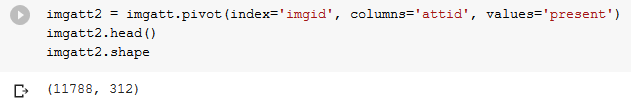
\includegraphics[width=8 cm]{figures/1174006/chapter3/soalpraktek/4-3.PNG}
	\end{figure}

	Setelah menjadikan atribut menjadi kolom, hasilnya terdapat 11 ribu baris dan 312 kolom.

	\hfill\break
	\begin{figure}[H]
	\centering
		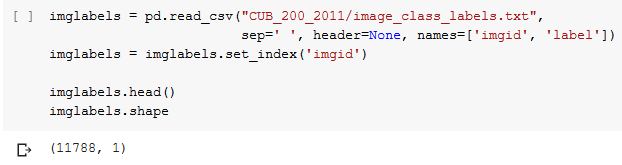
\includegraphics[width=8 cm]{figures/1174006/chapter3/soalpraktek/4-4.PNG}
	\end{figure}

	Setelah gambar burung diklasifikasikan sesuai dengan spesies labelnya, hasilnya terdapat 11 ribu baris dan 1 kolom saja.

	\hfill\break
	\begin{figure}[H]
	\centering
		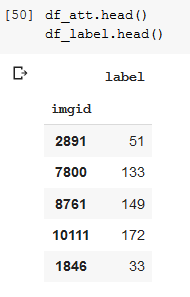
\includegraphics[width=8 cm]{figures/1174006/chapter3/soalpraktek/4-5.PNG}
	\end{figure}

	Menampilkan atribut dan label 5 bari data pertama.

	\hfill\break
	\begin{figure}[H]
	\centering
		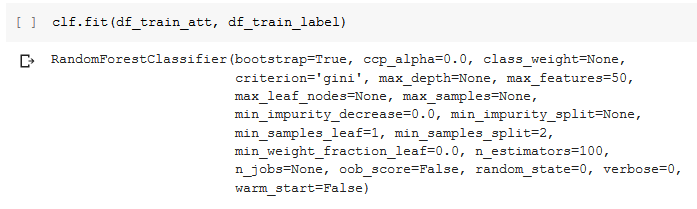
\includegraphics[width=8 cm]{figures/1174006/chapter3/soalpraktek/4-6.PNG}
	\end{figure}

	Dilakukan training dengan menggunakan metode Random Forest.

	\hfill\break
	\begin{figure}[H]
	\centering
		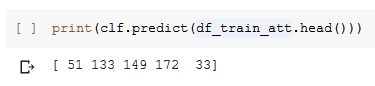
\includegraphics[width=8 cm]{figures/1174006/chapter3/soalpraktek/4-7.PNG}
	\end{figure}

	Menampilkan hasil prediksi dari 5 baris pertama.

	\hfill\break
	\begin{figure}[H]
	\centering
		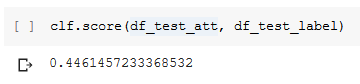
\includegraphics[width=8 cm]{figures/1174006/chapter3/soalpraktek/4-8.PNG}
	\end{figure}

	Akurasi yang didapat berjumlah 0.44\%.
	
	\item  Jalankan program confusion matrix pada bagian teori bab ini.  Tunjukkan kelu-arannya dari komputer sendiri dan artikan maksud setiap luaran yang didapatkan.
	
	\hfill\break
	\begin{figure}[H]
	\centering
		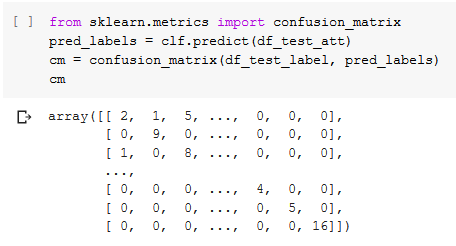
\includegraphics[width=8 cm]{figures/1174006/chapter3/soalpraktek/5-1.PNG}
	\end{figure}

	Menampilkan confusion matrix.

	\hfill\break
	\begin{figure}[H]
	\centering
		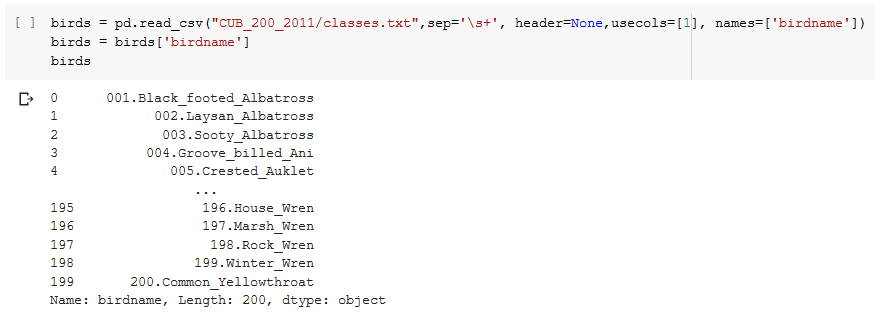
\includegraphics[width=8 cm]{figures/1174006/chapter3/soalpraktek/5-2.PNG}
	\end{figure}

	Menampilkan nama burung berdasarkan label klasifikasinya.

	\hfill\break
	\begin{figure}[H]
	\centering
		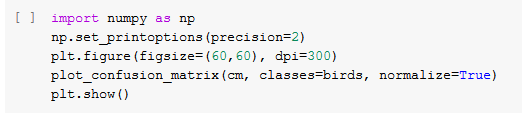
\includegraphics[width=8 cm]{figures/1174006/chapter3/soalpraktek/5-3-1.PNG}
	\end{figure}

	\begin{figure}[H]
	\centering
		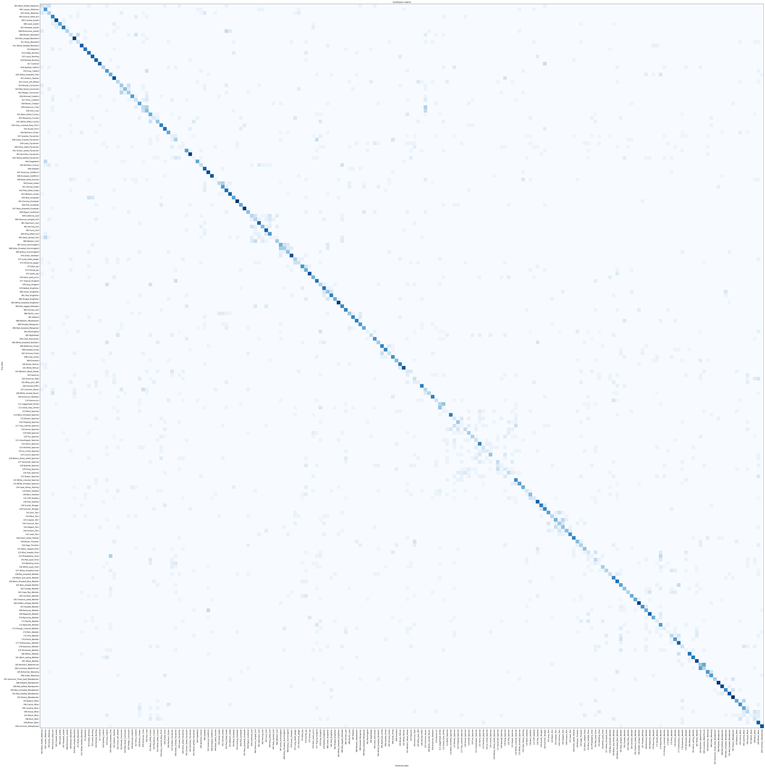
\includegraphics[width=8 cm]{figures/1174006/chapter3/soalpraktek/5-3-2.PNG}
	\end{figure}

	Membuat plot berdasarkan cofusion matrix.
	Jika diperbesar maka akan terlihat sumbu x adalah burung yang diprediksi dan sumbu y adalah burung yang sebenarnya.
	
	\item Jalankan  program  klasifikasi  SVM  dan  Decission  Tree  pada  bagian  teori  babini.  Tunjukkan keluarannya dari komputer sendiri dan artikan maksud setiapluaran yang didapatkan.
	
	\hfill\break
	\begin{figure}[H]
	\centering
		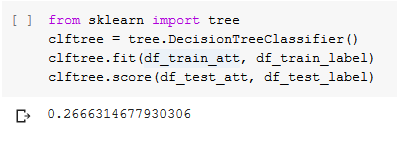
\includegraphics[width=8 cm]{figures/1174006/chapter3/soalpraktek/6-1.PNG}
	\end{figure}

	Menampilkan hasil akurasi dari decission tree.

	\hfill\break
	\begin{figure}[H]
	\centering
		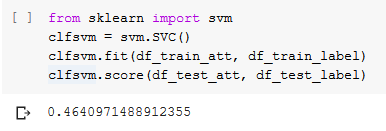
\includegraphics[width=8 cm]{figures/1174006/chapter3/soalpraktek/6-2.PNG}
	\end{figure}

	Menampilkan hasil akurasi dari SVM.
	
	\item Jalankan program cross validaiton pada bagian teori bab ini.  Tunjukkan kelu-arannya dari komputer sendiri dan artikan maksud setiap luaran yang didapatkan.
	
	\hfill\break
	\begin{figure}[H]
	\centering
		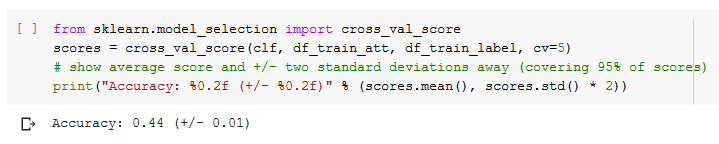
\includegraphics[width=8 cm]{figures/1174006/chapter3/soalpraktek/7-1.PNG}
	\end{figure}

	Menampilkan hasil validasi/evaluasi dari penggunaan random forest.

	\hfill\break
	\begin{figure}[H]
	\centering
		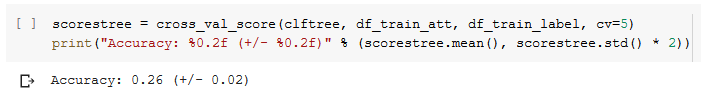
\includegraphics[width=8 cm]{figures/1174006/chapter3/soalpraktek/7-2.PNG}
	\end{figure}

	Menampilkan hasil validasi/evaluasi dari penggunaan decission tree.

	\hfill\break
	\begin{figure}[H]
	\centering
		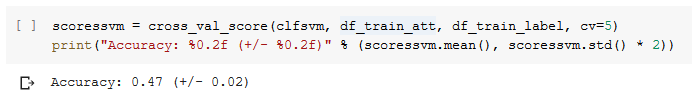
\includegraphics[width=8 cm]{figures/1174006/chapter3/soalpraktek/7-3.PNG}
	\end{figure}

	Menampilkan hasil validasi/evaluasi dari penggunaan SVM
	
	\item Jalankan program pengamatan komponen informasi pada bagian teori bab ini.Tunjukkan keluarannya dari komputer sendiri dan artikan maksud setiap luaran yang didapatkan.
	
	\hfill\break
	\begin{figure}[H]
	\centering
		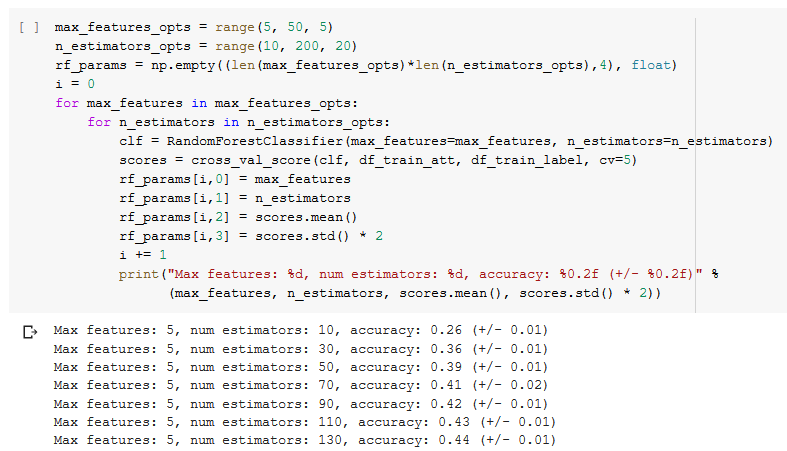
\includegraphics[width=8 cm]{figures/1174006/chapter3/soalpraktek/8-1.PNG}
	\end{figure}

	Melakukan evaluasi dari penggunaan Random Forest.

	\hfill\break
	\begin{figure}[H]
	\centering
		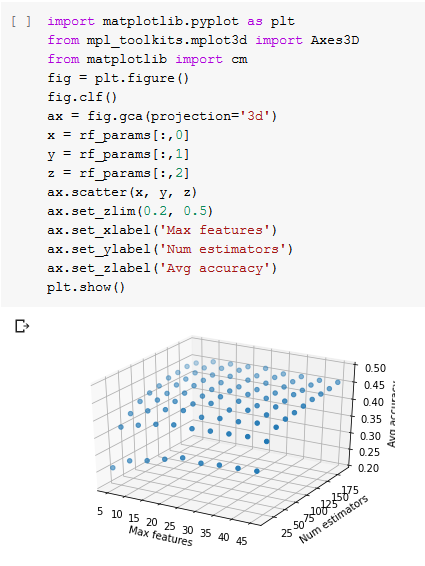
\includegraphics[width=8 cm]{figures/1174006/chapter3/soalpraktek/8-2.PNG}
	\end{figure}

	Memvisualisasikan hasil dari evaluasi dari penggunaan Random Forest.
	
\end{enumerate}

\subsection{Penanganan Error}
\begin{enumerate}
	\item Skrinsut error.
	\begin{itemize}
		\item Name Error
		\hfill\break
		\begin{figure}[H]
			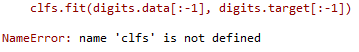
\includegraphics[width=8 cm]{figures/1174006/chapter1/error/err3.PNG}
			\centering
			\caption{Name Error.}
		\end{figure}
		\item Import Error
		\hfill\break
		\begin{figure}[H]
			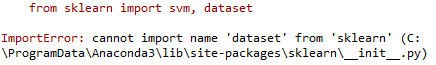
\includegraphics[width=8 cm]{figures/1174006/chapter1/error/err1.PNG}
			\centering
			\caption{Import Error.}
		\end{figure}
		\item Value Error
		\hfill\break
		\begin{figure}[H]
			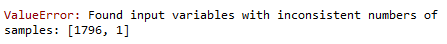
\includegraphics[width=8 cm]{figures/1174006/chapter1/error/err2.PNG}
			\centering
			\caption{Value Error.}
		\end{figure}
		\item Syntax Error
		\hfill\break
		\begin{figure}[H]
			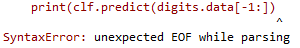
\includegraphics[width=8 cm]{figures/1174006/chapter1/error/err4.PNG}
			\centering
			\caption{Syntax Error.}
		\end{figure}
	\end{itemize}
	\item Tuliskan kode eror dan jenis errornya.
	\begin{itemize}
		\item Name Error
		\hfill\break
		Name Error adalah exception yang terjadi saat syntax melakukan eksekusi terhadap local name atau global name yang tidak terdefinisi.
		\item Import Error
		\hfill\break
		Import Error adalah exception yang terjadi saat syntax melakukan import terhadap library yang tidak terdefinisi.
		\item Value Error
		\hfill\break
		Value Error adalah exception yang terjadi saat syntax memiliki nilai yang tidak valid.
		\item Syntax Error
		\hfill\break
		Syntax Error adalah exception yang terjadi saat ada kesalahan dalam mengetikkan syntax.
	\end{itemize}
	\item Solusi pemecahan masalah error tersebut.
	\begin{itemize}
		\item Name Error
		\hfill\break
		Solusinya adalah memastikan variabel atau function yang dipanggil ada atau tidak salah ketik.
		\item Import Error
		\hfill\break
		Solusinya adalah memastikan library yang dipanggil ada atau tidak salah ketik.
		\item Value Error
		\hfill\break
		Solusinya adalah memastikan nilai yang diinputkan valid.
		\item Syntax Error
		\hfill\break
		Solusinya adalah memastikan syntax yang diketik tidak salah ketik.
	\end{itemize}
\end{enumerate}

\subsection{Bukti Tidak Plagiat}
\begin{figure}[H]
	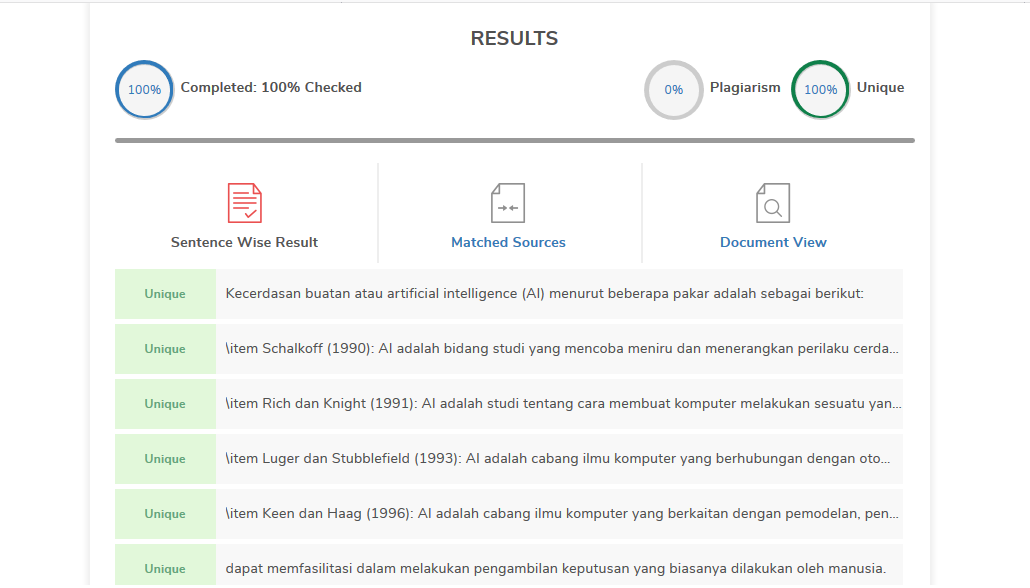
\includegraphics[width=8 cm]{figures/1174006/chapter1/plagiat.png}
	\centering
	\caption{Bukti Tidak Plagiat.}
\end{figure}